\section {Results}
\label{sec:results}

The classifers developed in this replication attempt were constructed and evaluated according to the parameters
and metrics described in Section~\ref{sec:modelflex}. Figure~\ref{fig:7_class_model} shows the sensitivity
and specificity of each tested model alongside the performance of the originally published model, with 10\% of models
most closely matching performance to the reference highlighted.
Tables~\ref{tab:prob_7class} and~\ref{tab:prob_8class} contain the complete performance of the probability-based models
evaluated using each performance metric for the 7- and 8-class settings, respectively. Table~\ref{tab:scikit_pred}
shows the same for the SKlearn Prediction models.

Finally, Table~\ref{tab:all_feature_performance} shows the evaluation
of the best-performing models fit on AAC when applied across all features.
\GK{For Hamid: regenerate data in the all-feature-performance table based on more than just the "best" model. At
present, we cannot include anything in the results about this because there isn't a result to discuss.}

The remainder of this section will explore the differences in model performance based on the defined axes of
flexibility enumerated in Section~\ref{sec:experimentaldesign}.

% Figure 1
\begin{figure}
  \centering
  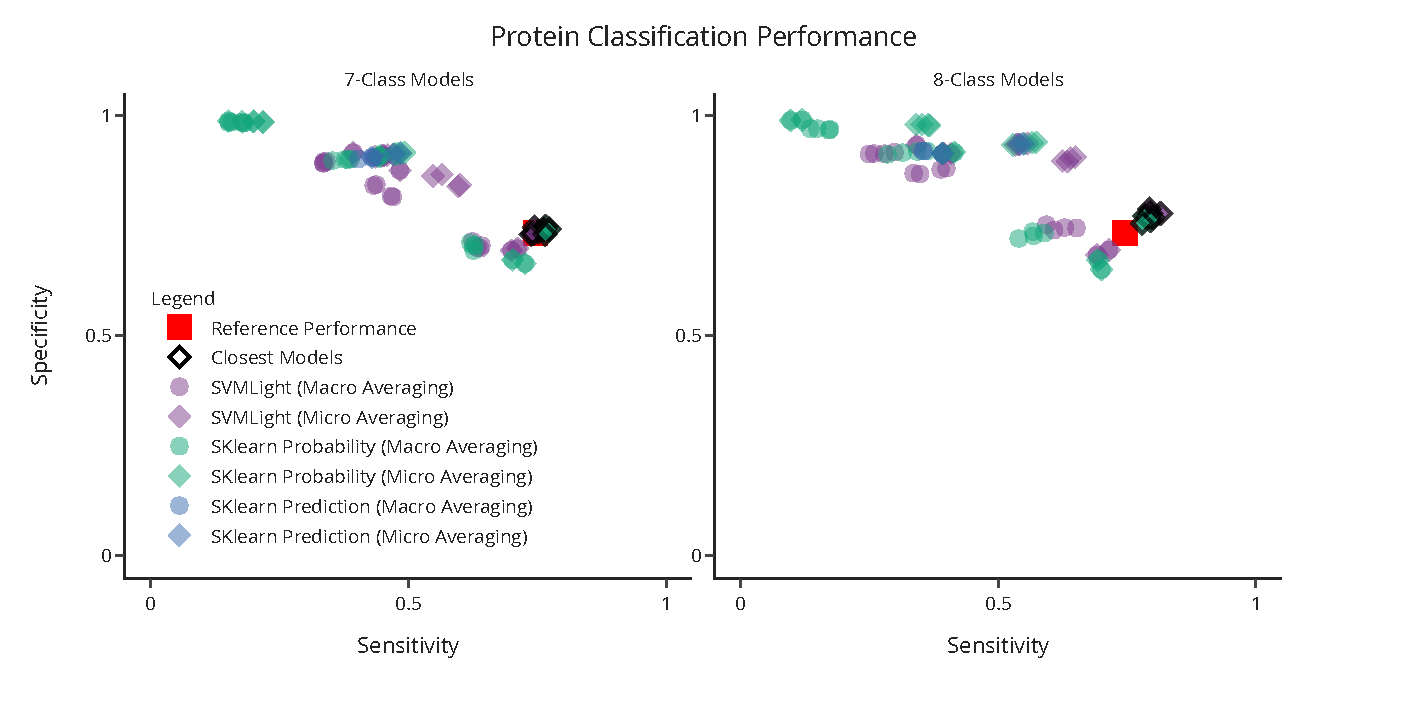
\includegraphics[width=\textwidth]{figures/fig1_model_performance.pdf}
  \caption{Sensitivity and Specificity of each tested model. Each panel contains models trained with a fixed number of
categories (7: left; 8: right), and shows the published reference performance in red. The closest 10\% of models to
this reference have been outlined in black. The symbol colour and shape refer to the classifier type and aggregation
strategy, respectively. Each shaded region illustrates the bounds of performance for a given binary classifier
aggregation strategy.}
   \label{fig:7_class_model}
\end{figure}

\paragraph{Number of Classes}
While the 7-class models appear to be slightly closer to the reference, there was no significant difference between
the number of classes and the distance from reference ($p > 0.1$). Models trained with 8 classes tended to achieve
higher sensitivity and specificity values, however, suggested improved performance with the addition of the background
class. 

\paragraph{Dataset Sampling}
The dataset composition had no significant impact on the closeness of the model to the reference ($p > 0.1$ for all
comparisons). However, none of the closest 10\% of models were trained using the downsampled dataset.

\paragraph{SVM Hyperparameters}
All uniformly parameterized models converged to same set of hyperparameters within the number of classes, where the
best performing 7-class models used Gamma and Cost values of $0.02$ and $4.5$ while 8-class models had best performance
with $0.01$ and $4$, respectively. There was no significant difference between these sets of parameters.

\paragraph{Hypterparamter Heterogeneity}
Similarly to the case of uniform parameters, models converged on Gamma values between $0.02$ and $0.04$ for all classes
and models, and Cost values between $4$ and $5$, with no statistically significant difference between models or classes.

\paragraph{Aggregation Technique}
Models using the micro performance-aggregation technique (i.e. evaluating individual binary classifiers prior to
aggregation into a multi-class classifier) obtained closer results to the reference than those using the macro
technique ($p < 1\times 10^{-4}$). All of the closest models used micro-aggregation.

\paragraph{Prediction Method}
The balanced averaging prediction method produced significantly closer results to the reference than both the
unweighted average and maximum probability methods ($p < 1\times 10^{-5}$ for both). The maximum probability method
also produced significantly closer results than the unweighted average method ($p < 0.001$).

\paragraph{Tool}
The SVMLight classifiers produced closer results to the reference than both SKlearn Probability and Prediction models
($p < 0.05$ for both). While the SKlearn Prediction model architecture did not appear in the set of closest models,
there was no statistically significant difference between its performance and that of the SKlearn Probability models.

\subsection{Closest Models}
The closest 10\% of models (16) used a variety of configurations, and each reported a distance score of less than
$0.13$ from the reference. The breakdown of configurations for these models included: micro aggregation (all), balanced
average prediction method (all), balanced (8) or shuffled (8) dataset, contained 7 (8) or 8 (8) classes in the dataset,
were trained with uniform (8) or heterogeneous (8) hyperparameters, and were developed using SVMLight (8) or the
SKlearn Probability (8) model architectures. While the SKlearn Prediction model and downsampled dataset configuration
are notably absent from these models, all other settings were either dominated by a single value, such as in the case
of micro aggregation and the balanced average prediction method, or the settings were equally represented. This
uniformity in representation is consistent with the direct comparisons between settings described above.

\GK{TODO Hamid: add results for the other analyses, such as 1- running the best 10\% of models on more features and
2- evaluating them on the independent dataset.}

% Table 1
\begin{table}[ht]
\begin{adjustwidth}{-2.25in}{0in} % Comment out/remove adjustwidth environment if table fits in text column.
    \centering
    \begin{tabular}{|L | V |V V V V g g g V V V V | V |}
        \hline
        \multicolumn{14}{|g|}{7-class based model for AAC}\\
        \hline
        \multicolumn{1}{|l|}{\multirow{2}{*}{\footnotesize{Original Results}}}
        &
        \multicolumn{3}{g}{Accuracy} & \multicolumn{3}{g}{Sensitivity} &
        \multicolumn{3}{g}{Specificity} & \multicolumn{4}{g|}{MCC}\\
        \cline{2-14}&
        \multicolumn{3}{C}{73.74} & \multicolumn{3}{C}{74.65} &
        \multicolumn{3}{C}{73.22} & \multicolumn{4}{C|}{0.46} \\
        \hline\hline
        
        \multicolumn{14}{|g|} {SVM Light}\\
        \hline\hline
        
        \cline{1-12}\multicolumn{1}{|g}{}&
        
        \multicolumn{1}{|g|}{\footnotesize{Dist}}&
        \multicolumn{4}{g} {\footnotesize{Gamma-Cost different for each class}}&
        \multicolumn{3}{g}{}&
        \multicolumn{4}{g|} {\footnotesize{same Gamma-Cost for all classes}}&
        \multicolumn{1}{g|}{\footnotesize{Dist}}\\
        
        \cline{3-6}\cline{10-13}\multicolumn{1}{|g}{}&
        \multicolumn{1}{|g|}{\footnotesize{ance}}&
        \multicolumn{1}{g}{acc}&\multicolumn{1}{g}{sens}&
        \multicolumn{1}{g}{spec}&\multicolumn{1}{g}{mcc}&
        \multicolumn{3}{g}{}&
        \multicolumn{1}{g}{acc}&\multicolumn{1}{g}{sens}&
        \multicolumn{1}{g}{spec}&\multicolumn{1}{g|}{mcc}&\multicolumn{1}{g|}{\footnotesize{ance}}\\

        \hline
        % \multicolumn{1}{|l|}{\multirow{6}{*}{\footnotesize{unweighted average}}}
        & 0.25 & 82.28 & 56.53 & 86.58 & 0.37 &    b&&b                & 80.73 & 60.00 & 84.18 & 0.37 & 0.21 \\
        & 0.43 & 84.07 & 39.28 & 91.55 & 0.32 &    d&\footnotesize{Micro}&d   & 81.90 & 48.33 & 87.5 & 0.32 & 0.33 \\
        \multicolumn{1}{|c|}{\multirow{1}{*}{\footnotesize{unweighted}}}
        & 0.26 & 81.74 & 54.74 & 86.24 & 0.36 &    s&&s                & 80.42 & 59.61 & 83.88 & 0.36 & 0.21 \\
        
        \cline{2-5}\cline{7-9}\cline{11-14}
        
        \multicolumn{1}{|c|}{\multirow{1}{*}{\footnotesize{average}}}
        & 0.37 & 82.28 & 43.76 & 84.31 & 0.31 &    b&&b                & 80.73 & 46.64 & 81.69 & 0.30 & 0.33 \\
        & 0.43 & 84.08 & 39.28 & 91.54 & 0.32 &    d&\footnotesize{Macro}&d   & 81.90 & 48.33 & 87.49 & 0.33 & 0.33 \\
        & 0.38 & 81.73 & 43.27 & 84.06 & 0.28 &    s&&s                & 80.42 & 46.96 & 81.49 & 0.29 & 0.33 \\
        
        \hline
        % \multicolumn{1}{|l|}{\multirow{6}{*}{\footnotesize{balanced average}}}
        &\mrkm{0.09}{73.84}{75.25}{73.60}{0.36} &    b&&b                & \mrkm{74.10}{75.12}{73.93}{0.36}{0.09} \\
        & 0.18 & 69.45 & 70.00 & 69.36 & 0.28 &     d&\footnotesize{Micro}&d   & 69.96 & 71.19 & 69.76 & 0.29 & 0.16 \\
        \multicolumn{1}{|c|}{\multirow{1}{*}{\footnotesize{balanced}}}
        &\mrkm{0.11}{72.06}{76.15}{71.39}{0.34} &    s&&s                &\mrkm{72.91}{75.38}{72.50}{0.35}{0.13} \\
        
        \cline{2-5}\cline{7-9}\cline{11-14}
        \multicolumn{1}{|c|}{\multirow{1}{*}{\footnotesize{average}}}
        & 0.20 & 73.84 & 64.18 & 70.45 & 0.28 &    b&&b                & 74.10 & 63.42 & 70.70 & 0.28 &  0.21 \\
        & 0.18 & 69.45 & 70.00 & 69.36 & 0.28 &     d&\footnotesize{Macro}&d   & 69.96 & 71.19 & 69.76 & 0.30 & 0.16 \\
        & 0.20 & 72.06 & 66.89 & 68.16 & 0.27 &     s&&s                & 72.91 & 64.46 & 69.24 & 0.26 & 0.21 \\
        
        \hline
        % \multicolumn{1}{|l|}{\multirow{6}{*}{\footnotesize{maximum probability}}}
        & 0.35 & 84.87 & 47.05 & 91.17 & 0.38 &    b&&b                & 84.54 & 45.89 & 90.98 & 0.36 & 0.36 \\
        & 0.37 & 84.35 & 45.24 & 90.87 & 0.36 &    d&\footnotesize{Micro}&d   & 83.87 & 43.57 & 90.59 & 0.34 & 0.38 \\
        \multicolumn{1}{|c|}{\multirow{1}{*}{\footnotesize{maximum}}}
        & 0.37 & 84.32 & 45.12 & 90.85 & 0.35 &    s&&s                & 84.21 & 44.74 & 90.79 & 0.35 & 0.37 \\
        
        \cline{2-5}\cline{7-9}\cline{11-14}

        \multicolumn{1}{|c|}{\multirow{1}{*}{\footnotesize{probability}}}
        & 0.48 & 84.87 & 34.05 & 89.58 & 0.28 &    b&&b                & 84.54 & 33.59 & 89.48 & 0.27 & 0.49 \\
        & 0.37 & 84.35 & 45.23 & 90.87 & 0.34 &    d&\footnotesize{Macro}&d   & 83.87 & 43.57 & 90.59 & 0.33 & 0.39 \\
        & 0.48 & 84.32 & 33.52 & 89.14 & 0.27 &    s&&s                & 84.21 & 33.47 & 89.15 & 0.27 & 0.48 \\
        
        \hline\hline
        
        \multicolumn{14}{|g|} {Scikit Learn}\\
        \hline\hline

        % \multicolumn{1}{|l|}{\multirow{6}{*}{\footnotesize{unweighted average}}}
        & 0.61 & 87.51 & 21.47 & 98.44 & 0.33 &    b&&b                 & 87.45 & 19.39 & 98.69 & 0.32 & 0.63 \\
        & 0.65 & 87.03 & 17.43 & 98.60 & 0.29 &    d&\footnotesize{Micro}&d   & 86.68 & 15.28 & 98.56 & 0.27 & 0.68 \\
        \multicolumn{1}{|c|}{\multirow{1}{*}{\footnotesize{unweighted}}}
        & 0.61 & 87.49 & 21.66 & 98.41 & 0.34 &    s&&s                & 87.55 & 20.878 & 98.63 & 0.34 & 0.62 \\
        
        \cline{2-5}\cline{7-9}\cline{11-14}

        \multicolumn{1}{|c|}{\multirow{1}{*}{\footnotesize{average}}}
        & 0.66 & 87.49 & 18.29 & 98.20 & 0.24 &    b&&b                 & 87.44 & 14.87 & 98.46 & 0.20 & 0.71 \\
        & 0.67 & 87.03 & 17.46 & 98.61 & 0.24 &    d&\footnotesize{Macro}&d   & 86.68 & 15.32 & 98.56 & 0.22 & 0.70 \\
        & 0.67 & 87.47 & 17.52 & 98.18 & 0.23 &    s&&s                & 87.53 & 16.32 & 98.40 & 0.21 & 0.69 \\
        
        \hline
        % \multicolumn{1}{|l|}{\multirow{6}{*}{\footnotesize{balanced average}}}
        & \mrkm{0.07}{75.33}{76.42}{75.13}{0.38} &    b&&b                 & \mrkm{75.33}{76.41}{75.15}{0.38}{0.07} \\
        & 0.20 & 68.09 & 70.95 & 67.62 & 0.27 &    d&\footnotesize{Micro}&d   & 67.31 & 70.47 & 66.78 & 0.26 & 0.21 \\
        \multicolumn{1}{|c|}{\multirow{1}{*}{\footnotesize{balanced}}}
        & \mrkm{0.07}{75.32}{76.41}{75.15}{0.38} &    s&&s                & \mrkm{73.46}{75.25}{73.16}{0.35}{0.10} \\
        
        \cline{2-5}\cline{7-9}\cline{11-14}
        
        \multicolumn{1}{|c|}{\multirow{1}{*}{\footnotesize{average}}}
        & 0.20 & 75.32 & 61.79 & 71.51 & 0.29 &    b&&b                 & 75.32 & 61.79 & 71.51 & 0.30 & 0.20 \\
        & 0.18 & 68.09 & 70.95 & 67.61 & 0.29 &    d&\footnotesize{Macro}&d   & 67.31 & 70.47 & 66.78 & 0.27 & 0.20 \\
        & 0.20 & 75.32 & 61.79 & 71.22 & 0.29 &    s&&s                & 73.46 & 61.48 & 69.51 & 0.25 & 0.24 \\
        
        \hline
        % \multicolumn{1}{|l|}{\multirow{6}{*}{\footnotesize{maximum probability}}}
        & 0.34 & 85.38 & 48.84 & 91.47 & 0.40 &    b&&b          & 85.20 & 48.20 & 91.36 & 0.39 & 0.34 \\
        & 0.37 & 84.21 & 44.76 & 90.79 & 0.35 &    d&\footnotesize{Micro}&d   & 84.14 & 44.52 & 90.75 & 0.35 & 0.37 \\
        \multicolumn{1}{|c|}{\multirow{1}{*}{\footnotesize{maximum}}}
        & 0.34 & 85.12 & 47.95 & 91.32 & 0.39 &    s&&s                & 85.12 & 47.94 & 91.32 & 0.39 & 0.34 \\
        
        \cline{2-5}\cline{7-9}\cline{11-14}
        \multicolumn{1}{|c|}{\multirow{1}{*}{\footnotesize{probability}}}
        & 0.43 & 85.38 & 38.43 & 89.98 & 0.32 &    b&&b                 & 85.20 & 37.61 & 89.90 & 0.31 & 0.44 \\
        & 0.38 & 84.21 & 44.76 & 90.79 & 0.32 &    d&\footnotesize{Macro}&d   & 84.14 & 44.52 & 90.75 & 0.33 & 0.38 \\
        & 0.44 & 85.12 & 38.33 & 89.94 & 0.31 &    s&&s                & 85.12 & 36.43 & 89.85 & 0.30 & 0.46 \\
        \hline\hline
        
        \multicolumn{14}{|c|} {\footnotesize{
            B, D and S are balanced, down-sampled and shuffled instances of the main dataset.
        }}\\
        \multicolumn{14}{|c|} {\footnotesize{
            Acc: Accuracy, Sens: Sensitivity, Spec: Specificity, Mcc: Matthews correlation coefficient
        }}\\

        \hline
        
       

    \end{tabular}
    \captionsetup{font=small,width=14cm}
    \caption{The average sensitivity, specificity, accuracy, and MCC  for 7 class-based models.}
    \label{tab:prob_7class}
\end{adjustwidth}    
\end{table}

\begin{table}[ht]
\begin{adjustwidth}{-2.25in}{0in} % Comment out/remove adjustwidth environment if table fits in text column.
    \centering
    \begin{tabular}{|L | V |V V V V g g g V V V V | V |}
        \hline
        \multicolumn{14}{|g|}{8-class based model for AAC}\\
        \hline
        \multicolumn{1}{|l|}{\multirow{2}{*}{\footnotesize{Original Results}}}
        &
        \multicolumn{3}{g}{Accuracy} & \multicolumn{3}{g}{Sensitivity} &
        \multicolumn{3}{g}{Specificity} & \multicolumn{4}{g|}{MCC}\\
        \cline{2-14}&
        \multicolumn{3}{C}{73.74} & \multicolumn{3}{C}{74.65} &
        \multicolumn{3}{C}{73.22} & \multicolumn{4}{C|}{0.46} \\
        \hline\hline
        
        \multicolumn{14}{|g|} {SVM Light}\\
        \hline\hline
        
        \cline{1-12}\multicolumn{1}{|g}{}&
        
        \multicolumn{1}{|g|}{\footnotesize{Dist}}&
        \multicolumn{4}{g} {Gamma-Cost different for each class}&
        \multicolumn{3}{g}{}&
        \multicolumn{4}{g|} {same Gamma-Cost for all classes}&
        \multicolumn{1}{g|}{\footnotesize{Dist}}\\
        
        \cline{3-6}\cline{10-13}\multicolumn{1}{|g}{}&
        \multicolumn{1}{|g|}{\footnotesize{ance}}&
        \multicolumn{1}{g}{acc}&\multicolumn{1}{g}{sens}&
        \multicolumn{1}{g}{spec}&\multicolumn{1}{g}{mcc}&
        \multicolumn{3}{g}{}&
        \multicolumn{1}{g}{acc}&\multicolumn{1}{g}{sens}&
        \multicolumn{1}{g}{spec}&\multicolumn{1}{g|}{mcc}&\multicolumn{1}{g|}{\footnotesize{ance}}\\

        \hline

        % \multicolumn{1}{|l|}{\multirow{6}{*}{\footnotesize{unweighted average}}}
        
        & 0.24 & 87.33 & 64.92 & 90.53 & {0.49} &    b&&b               & 86.22 & 63.40 & 89.48 & 0.46 & 0.23 \\
        & 0.49 & 85.86 & 34.16 & 93.24 & 0.30 &    d&\footnotesize{Micro}&d   & 85.02 & 40.83 & 91.34 & 0.32 & 0.42 \\
        \multicolumn{1}{|c|}{\multirow{1}{*}{\footnotesize{unweighted}}}
        & 0.24 & 87.02 & 63.98 & 90.31 & 0.48 &    s&&s                & 86.24 & 62.46 & 89.63 & 0.46 & 0.23 \\
        
        \cline{2-5}\cline{7-9}\cline{11-14}
        
        \multicolumn{1}{|c|}{\multirow{1}{*}{\footnotesize{average}}}
        & 0.43 & 87.33 & 39.91 & 88.02 & 0.30 &    b&&b               & 86.22 & 34.78 & 86.71 & 0.25 & 0.48 \\
        & 0.49 & 85.85 & 34.16 & 93.24 & 0.28 &    d&\footnotesize{Macro}&d   & 85.02 & 40.83 & 91.34 & 0.30 & 0.42 \\
        & 0.44 & 87.02 & 38.81 & 87.71 & 0.28 &    s&&s                & 86.24 & 33.57 & 86.89 & 0.23 & 0.50 \\
        
        \hline
        % \multicolumn{1}{|l|}{\multirow{6}{*}{\footnotesize{balanced average}}}

        & \mrkm{0.10}{79.98}{79.78}{80.01}{0.44} &    b&&b               & \mrkm{79.74}{77.97}{80.00}{0.43}{0.10} \\
        & 0.19 & 68.93 & 71.87 & 68.51 & 0.27 &     d&\footnotesize{Micro}&d   & 68.07 & 69.79 & 67.82 & 0.25 & 0.22 \\
        \multicolumn{1}{|c|}{\multirow{1}{*}{\footnotesize{balanced}}}
        & \mrkm{0.09}{77.71}{79.93}{77.40}{0.41} &     s&&s                & \mrkm{78.31}{78.33}{78.31}{0.41}{0.09} \\
        
        \cline{2-5}\cline{7-9}\cline{11-14}

        \multicolumn{1}{|c|}{\multirow{1}{*}{\footnotesize{average}}}
        & 0.21 & 79.59 & 57.34 & 76.24 & 0.28 &    b&&b               & 79.59 & 57.34 & 76.24 & 0.28 & 0.25 \\
        & 0.19 & 68.93 & 71.87 & 68.51 & 0.27 &     d&\footnotesize{Macro}&d   & 68.07 & 69.79 & 67.82 & 0.25 & 0.22 \\
        & 0.21 & 77.71 & 53.55 & 74.14 & 0.27 &     s&&s                & 78.31 & 58.42 & 74.72 & 0.26. & 0.26 \\
        
        \hline
        % \multicolumn{1}{|l|}{\multirow{6}{*}{\footnotesize{maximum probability}}}

        & 0.31 & 88.91 & 55.65 & 93.66 & {0.49} &    b&&b               & 88.51 & 54.05 & 93.43 & 0.47 & 0.32 \\
        & 0.43 & 84.84 & 39.37 & 91.33 & 0.30 &    d&\footnotesize{Micro}&d   & 84.79 & 39.16 & 91.30 & 0.30 & 0.44 \\
        \multicolumn{1}{|c|}{\multirow{1}{*}{\footnotesize{maximum}}}
        & 0.32 & 88.44 & 53.76 & 93.39 & 0.47 &    s&&s                & 88.33 & 53.33 & 93.33 & 0.46 & 0.32 \\
        
        \cline{2-5}\cline{7-9}\cline{11-14}

        \multicolumn{1}{|c|}{\multirow{1}{*}{\footnotesize{probability}}}
        & 0.54 & 88.91 & 29.87 & 91.65 & 0.26 &    b&&b               & 88.51 & 25.93 & 91.35 & 0.22 & 0.58 \\
        & 0.44 & 84.84 & 39.37 & 91.34 & 0.29 &    d&\footnotesize{Macro}&d   & 84.79 & 39.16 & 91.31 & 0.28 & 0.44 \\
        & 0.57 & 88.44 & 27.85 & 91.28 & 0.23 &    s&&s                & 88.33 & 24.93 & 91.22 & 0.20 & 0.60 \\
        
        \hline
        \hline
        
        \multicolumn{14}{|g|} {Scikit Learn}\\
        \hline
        \hline

        % \multicolumn{1}{|l|}{\multirow{6}{*}{\footnotesize{unweighted average}}}
        
        & 0.48 & 90.22 & 36.33 & 97.84 & 0.46  &    b&&b               & 90.11 & 35.22 & 97.92 & 0.45 & 0.49 \\
        & 0.72 & 88.10 & 12.18 & 98.86 & 0.23 &    d&\footnotesize{Micro}&d   & 87.75 & 9.63 & 98.86 & 0.19 & 0.76  \\
        \multicolumn{1}{|c|}{\multirow{1}{*}{\footnotesize{unweighted}}}
        & 0.48 & 90.10 & 36.52 & 97.68 & 0.45 &    s&&s                & 89.89 & 33.28 & 97.96 & 0.43 & 0.50 \\
        
        \cline{2-5}\cline{7-9}\cline{11-14}

        \multicolumn{1}{|c|}{\multirow{1}{*}{\footnotesize{average}}}
        & 0.68 & 90.19 & 17.30 & 96.85 & 0.22 &    b&&b               & 90.10 & 15.26 & 96.98 & 0.17 & 0.71 \\
        & 0.74 & 88.10 & 12.21 & 98.86 & 0.18 &    d&\footnotesize{Macro}&d   & 87.75 & 9.71 & 8.86 & 0.13 & 0.78  \\
        & 0.68 & 90.07 & 17.17 & 96.68 & 0.20 &    s&&s                & 89.88 & 12.90 & 97.02 & 0.15 & 0.74 \\
        
        \hline
        % \multicolumn{1}{|l|}{\multirow{6}{*}{\footnotesize{balanced average}}}

        & \mrkm{0.08}{77.08}{80.0}{76.66}{0.40}  &     b&&b               & \mrkm{77.70}{78.18}{77.63}{0.40}{0.08} \\
        & 0.22 & 67.91 & 69.16 & 67.73 & 0.25 &     d&\footnotesize{Micro}&d   & 68.75 & 67.28 & 68.96 & 0.25 & 0.23  \\
        \multicolumn{1}{|c|}{\multirow{1}{*}{\footnotesize{balanced}}}
        & \mrkm{0.08}{76.66}{78.47}{76.40}{0.39} &     s&&s                & \mrkm{74.36}{79.41}{73.64}{0.37}{0.09} \\
        
        \cline{2-5}\cline{7-9}\cline{11-14}

        \multicolumn{1}{|c|}{\multirow{1}{*}{\footnotesize{average}}}
        & 0.24 & 77.08 & 59.13 & 73.10 & 0.27 &     b&&b               & 77.70 & 54.72 & 74.14 & 0.25 & 0.28 \\
        & 0.21 & 67.91 & 69.16 & 67.73 & 0.26 &     d&\footnotesize{Macro}&d   & 68.75 & 67.29 & 68.95 & 0.26 & 0.22  \\
        & 0.27 & 76.66 & 56.55 & 72.78 & 0.25 &     s&&s                & 74.36 & 56.27 & 0.07 & 0.22 & 0.30 \\
        
        \hline
        % \multicolumn{1}{|l|}{\multirow{6}{*}{\footnotesize{maximum probability}}}

        & 0.31 & 89.33 & 57.31 & 93.90 & 0.51 &     b&&b         & 88.73 & 54.92 & 93.56 & 0.48 & 0.32 \\
        & 0.42 & 85.10 & 40.41 & 91.49 & 0.31 &     d&\footnotesize{Micro}&d   & 85.31 & 41.25 & 91.60 & 0.32 & 0.41  \\
        \multicolumn{1}{|c|}{\multirow{1}{*}{\footnotesize{maximum}}}
        & 0.31 & 89.09 & 56.37 & 93.76 & 0.50 &     s&&s                & 88.15 & 52.60 & 93.22 & 0.45 & 0.33 \\
        
        \cline{2-5}\cline{7-9}\cline{11-14}

        \multicolumn{1}{|c|}{\multirow{1}{*}{\footnotesize{probability}}}
        & 0.47 & 89.32 & 36.12 & 91.94 & 0.34 &     b&&b               & 88.73 & 31.39 & 91.51 & 0.29 & 0.52 \\
        & 0.43 & 85.10 & 40.41 & 91.48 & 0.30 &     d&\footnotesize{Macro}&d   & 85.31 & 41.25 & 91.60 & 0.31 & 0.42  \\
        & 0.49 & 89.09 & 33.78 & 91.73 & 0.30 &     s&&s                & 88.15 & 28.05 & 91.14 & 0.23 & 0.56 \\
        \hline\hline
        
        \multicolumn{14}{|c|} {\footnotesize{
            B, D and S are balanced, down-sampled and shuffled instances of the main dataset.
        }}\\
        \multicolumn{14}{|c|} {\footnotesize{
            Acc: Accuracy, Sens: Sensitivity, Spec: Specificity, Mcc: Matthews correlation coefficient
        }}\\

        \hline
        
       

    \end{tabular}
    \captionsetup{font=small,width=14cm}
    \caption{The average sensitivity, specificity, accuracy, and MCC  for 8 class-based models.}
    \label{tab:prob_8class}
    
\end{adjustwidth}
\end{table}




\begin{table}[ht]
\begin{adjustwidth}{-2.25in}{0in} % Comment out/remove adjustwidth environment if table fits in text column.
    \centering
    \begin{tabular}{|L | V |V V V V g g g V V V V | V |}
        \hline
        \multicolumn{14}{|g|}{Scikit-learn prediction-based models}\\
        \hline
        \multicolumn{1}{|l|}{\multirow{2}{*}{\footnotesize{Original Results}}}
        &
        \multicolumn{3}{g}{Accuracy} & \multicolumn{3}{g}{Sensitivity} &
        \multicolumn{3}{g}{Specificity} & \multicolumn{4}{g|}{MCC}\\
        \cline{2-14}&
        \multicolumn{3}{C}{73.74} & \multicolumn{3}{C}{74.65} &
        \multicolumn{3}{C}{73.22} & \multicolumn{4}{C|}{0.46} \\
        \hline
        
        \cline{1-12}\multicolumn{1}{|g}{}&
        
        \multicolumn{1}{|g|}{\footnotesize{Dist}}&
        \multicolumn{4}{g} {\footnotesize{7 class-based models}}&
        \multicolumn{3}{g}{}&
        \multicolumn{4}{g|} {\footnotesize{8 class-based models}}&
        \multicolumn{1}{g|}{\footnotesize{Dist}}\\
        
        \cline{3-6}\cline{10-13}\multicolumn{1}{|g}{}&
        \multicolumn{1}{|g|}{\footnotesize{ance}}&
        \multicolumn{1}{g}{acc}&\multicolumn{1}{g}{sens}&
        \multicolumn{1}{g}{spec}&\multicolumn{1}{g}{mcc}&
        \multicolumn{3}{g}{}&
        \multicolumn{1}{g}{acc}&\multicolumn{1}{g}{sens}&
        \multicolumn{1}{g}{spec}&\multicolumn{1}{g|}{mcc}&\multicolumn{1}{g|}{\footnotesize{ance}}\\

        \hline

        \multicolumn{1}{|l|}{\multirow{6}{*}{\footnotesize{Prediction-based}}}
        
        & 0.70 & 76.88 & 19.10 & 86.51 & 0.05 &    s&&s                & 84.58 & 38.33 & 91.19 & 0.29 & 0.45 \\
            & 0.39 & 83.66 & 42.86 & 90.47 & 0.33 &    d&\small{Micro}&d   & 84.79 & 39.16 & 91.31 & 0.30 & 0.44 \\
            & 0.36 & 84.43 & 45.51 & 90.91 & 0.36 &    sh&&sh              & 88.71 & 54.85 & 93.54 & 0.48 & 0.32 \\
    
            
            \cline{2-5}\cline{7-9}\cline{11-14}
            
            & 0.81 & 76.88 & 6.69 & 81.70 & 0.01 &    s&&s                & 84.58 & 76.82 & 86.79 & 0.03 & 0.81 \\
            & 0.39 & 83.67 & 42.85 & 90.47 & 0.32 &    d&\small{Macro}&d   & 84.79 & 39.16 & 91.31 & 0.29 & 0.44 \\
            & 0.39 & 85.27 & 43.31 & 90.33 & 0.35 &    sh&&sh              & 88.71 & 35.32 & 91.94 & 0.29 & 0.48 \\
        
        \hline\hline
        
        \multicolumn{14}{|c|} {\footnotesize{
            S, D and SH are sorted, down-sampled and shuffled instances of the main dataset.
        }}\\
        \multicolumn{14}{|c|} {\footnotesize{
            Acc: Accuracy, Sens: Sensitivity, Spec: Specificity, Mcc: Matthews correlation coefficient
        }}\\

        \hline
    \end{tabular}
    \captionsetup{font=small,width=14cm}
    \caption{The average sensitivity, specificity, accuracy, and MCC values 
    for scikit-learn prediction-based models for amino acid composition (AAC).}
    \label{tab:scikit_pred}
\end{adjustwidth}
\end{table}

\begin{table}[ht]
\begin{adjustwidth}{-2.25in}{0in} % Comment out/remove adjustwidth environment if table fits in text column.

    \centering

    \begin{tabular}{|L || g g g g || C C C C|}
    \hline
    \multicolumn{1}{|l||}{\multirow{2}{*}{Method}}
    &
    \multicolumn{4}{g||}{Paper's Results}
    &
    \multicolumn{4}{c|}{Reproduced Results}
    \\ \cline{2-5} \cline{6-9}
    \multicolumn{1}{|c||}{}
    &
    Sensitivity  &  Specificity  &  Accuracy  &  MCC
    &
    Sensitivity  &  Specificity  &  Accuracy  &  MCC
    \\
    \hline \hline
    AAC & 74.65 & 73.22 & 73.74 & 0.46      &    79.98 & 79.78 & 80.01 & 0.44 \\
    DPC & 71.36 & 71.17 & 71.32 & 0.40 & -- & -- & -- & --  \\
    PHC & 70.63 & 70.42 & 70.60 & 0.38 & -- & -- & -- & --  \\
    AAI & 71.54 & 71.98 & 71.80 & 0.40 & -- & -- & -- & --  \\
    PSSM & 74.00 & 76.03 & 75.48 & 0.47 & -- & -- & -- & --  \\
    \hline
    AAC + AAI & 73.84 & 73.36 & 73.37 & 0.44 & -- & -- & -- & --  \\
    AAC + PHC & 73.56 & 73.39 & 73.40 & 0.44 & -- & -- & -- & --  \\
    AAC + DPC & 73.01 & 74.23 & 73.85 & 0.44 & -- & -- & -- & --  \\
    AAC + PSSM & 72.33 &  74.62 &  73.87 &  0.44 & -- & -- & -- & --  \\
    DPC + PHC & 72.15 &73.13 &72.90 &0.43 & -- & -- & -- & --  \\
    DPC + AAI &    70.28  & 72.09 &  71.67 &  0.40 & -- & -- & -- & --  \\
    DPC + PSSM &69.87 &72.06 &71.37 &0.40& -- & -- & -- & --  \\
    AAI + PHC & 69.32 &  71.50 &  70.79 &  0.38 & -- & -- & -- & --  \\
    AAI + PSSM & 76.19 &77.17 &76.69& 0.49 & -- & -- & -- & -- \\
    \hline
    AAC + DPC + AAI & 73.01 &  74.32  & 73.89&   0.44 & -- & -- & -- & --  \\
    AAC + DPC + PHC & 73.04& 75.36   &74.75  & 0.46& -- & -- & -- & --  \\
    AAC + DPC + PSSM & 73.43 &73.73 &73.64 &0.44& -- & -- & -- & --  \\
    AAC + AAI + PHC & 73.01  & 73.82 &73.51 &  0.44& -- & -- & -- & --  \\
    AAC + AAI + PSSM & 72.34 &  74.62& 73.90 &  0.44 & -- & -- & -- & --  \\
    \hline
    \end{tabular}
    \captionsetup{font=small,width=12cm}
    \caption{The average sensitivity, specificity, accuracy, and MCC for all seven 
    substrate-specific transporter classes for different SVM models on main dataset 
    comparing original results with the results from our best reproduced model}
    \label{tab:all_feature_performance}
\end{adjustwidth}
\end{table}

